\documentclass[11pt]{article}

%\usepackage{fullpage}
\usepackage[margin=1in]{geometry}
\usepackage{epsfig, hyperref}
%\usepackage{mathptmx}
\usepackage{algorithm}
\usepackage{algpseudocode}
\usepackage{times}
\usepackage{amsmath, amsthm, amssymb}
\usepackage{tikz}
\newtheorem{theorem}{Theorem}
\newtheorem{claim}{Claim}
\newcommand{\eat}[1]{}

\newcommand{\cI}{{\cal I}}
\newcommand{\cA}{{\cal A}}
\newcommand{\cB}{{\cal B}}
\newcommand{\bigO}{{\cal O}}
\newcommand{\opt}{{\mathsf{opt}}}
\usepackage{color}
\newcommand{\alert}[1]{\textcolor{red}{#1}}
\newcommand{\poly}{{\rm poly}}
\newcommand{\cR}{{\mathsf{CR}}}
\newcommand{\mk}{{\textsc{MARKING }}}
\newcommand{\expt}[1]{{\mathbb E[#1]}}
\newcommand{\prob}[1]{{\mathbb P[#1]}}

\title{
    \textbf{CSE586: Algorithms Under Uncertainty} \\
    Homework 1 Solution % \\
    % Team Member 1: \href{mailto:ashlesha21380@iiitd.ac.in}{Ashlesha Gupta (2021380)} \\
    % Team Member 2: \href{mailto:divyajeet21529@iiitd.ac.in}{Divyajeet Singh (2021529)}
}
\author{
    \href{mailto:ashlesha21380@iiitd.ac.in}{Ashlesha Gupta (2021380)} \and
    \href{mailto:divyajeet21529@iiitd.ac.in}{Divyajeet Singh (2021529)}
}
\date{}

\begin{document}
\maketitle

\section*{Solution 1.}
We are given a sequence of purchase options $(d_{1}, p_{1})$, $(d_{2}, p_{2})$, $\hdots$, $(d_{k}, p_{k})$, and options $(1, 1)$
and $(\infty, B)$. It is also given that the options follow economies of scale, i.e.
\begin{equation}
    \label{eco}
    d_{1} < d_{2} < \cdots < d_{k} \implies \frac{p_{1}}{d_{1}} > \frac{p_{2}}{d_{2}} > \cdots > \frac{p_{k}}{d_{k}}
\end{equation}

\begin{claim}
    \label{claim:assumption}
    It is okay to assume that $p_{i-1} \leq \frac{p_{i}}{2}$ for all $2 \leq i \leq k$.
\end{claim}
\begin{quote}
\textit{Proof.}
Assume there exist purchase options $(d_{j-1}, p_{j-1})$ and $(d_{j}, p_{j})$ for some $2 \leq j \leq k$ such that
\begin{align}
    \label{skip-j-1}
    p_{j-1} &> \frac{p_{j}}{2} \\
    \label{days}
    d_{j-1} &< d_{j}
\end{align}
If it snows for $d_{j-1} < d \leq d_{j+1}$ days, then we can either select the purchase option $(d_{j}, p_{j})$
once or the purchase option $(d_{j-1}, p_{j-1})$ some $r$ times. By \eqref{days}, $r > 1$.
Let us assume we pick the second choice. Then, we pay
\begin{equation}
    r \cdot p_{j-1} \geq r \cdot \frac{p_{j}}{2} \geq p_{j}
\end{equation}
where the last inequality holds because $r \geq 2$. So, we end up paying more than the cost
of the purchase option $(d_{j}, p_{j})$. So, we would never pick the purchase option $(d_{j-1}, p_{j-1})$. \\
If it snows for more than $d_{j}$ days, then we can either select $(d_{j}, p_{j})$ some $r_{1}$ times or
$(d_{j-1}, p_{j-1})$ some $r_{2}$ times. By \eqref{days}, $r_{1} \leq r_{2}$. In this case, we pick $(d_{j}, p_{j})$ $r_{1}$
times because by \eqref{eco},
\begin{equation}
    \frac{p_{j}}{d_{j}} > \frac{p_{j-1}}{d_{j-1}}
\end{equation}
which means we get better value for money by picking $(d_{j}, p_{j})$ $r_{1}$ times. \\
Hence, it is safe to ignore $(d_{j-1}, p_{j-1})$ if \eqref{skip-j-1} doesn't hold.
\hfill $\square$
\end{quote}

\subsection*{Offline Optimal Algorithm}
The offline ski-rental problem with multiple purchase options can be solved using dynamic programming. Assuming it snows
for $T \leq |\sigma|$ days, for each day $1 \leq i \leq T$, we calculate the minimum cost of renting skiis for the
first $i$ days. The pseudocode for this algorithm is given in Algorithm \ref{alg:opt-ski-rental-1}.
\begin{algorithm}
    \caption{Offline Optimal Algorithm for modified the Ski-Rental Problem}
    \label{alg:opt-ski-rental-1}
    \begin{algorithmic}[1]
        \Procedure{Ski-rental}{$\sigma[1:N]$, $(d_{i}, p_{i})[1:k]$}:
            \State $T \gets \sum_{i=1}^{N}\sigma[i]$ \Comment{Total number of days it snows}
            \State $C[0:T] \gets \infty$
            \State $C[0] \gets 0$
            \For{$i \gets 1$ to $T$}
                \For{$j \gets 1$ to $i$}
                    \State $C[i] \gets \min{(C[i], C[i - d_{j}] + p_{j})}$
                \EndFor
                \State $C[i] \gets \min{(C[i], C[i - 1] + 1)}$ \Comment{Rent for $1$ day}
            \EndFor
            \State \Return $\min{(C[T], B)}$
        \EndProcedure
    \end{algorithmic}
\end{algorithm}
\vspace*{0pt} \\
The algorithm runs in $\bigO(T*k)$ time and $\bigO(T)$ space, meaning it is polynomial in the input size.

\subsection*{Competitive Online Algorithm}
Now, we design an algorithm to solve the online version of the modified ski-rental porblem. Without loss of generality,
we assume that the sequence of purchase options is sorted in increasing order of $d_{i}$'s, and that $(d_{1}, p_{1}) = (1, 1)$
and $(d_{k}, p_{k}) = (\infty, B)$ (Note how it does not affect our algorithm or its analysis). Finally, we assume that
\eqref{eco} and Claim \ref{claim:assumption} hold. \\
Our algorithm, $\mathbf{\Lambda}$, is a generalization of the simple online ski-rental problem. In that version, we have
two purchase options, $(1, 1)$ and $(\infty, B)$. The optimal strategy is to rent skiis (\textit{use} $(1, 1)$) for $B-1$ days and then
buy them (\textit{use} $(\infty, B)$) on the last day, unless it stops snowing. This suggests that we use the purchase option
$(d_{i}, p_{i})$ for $d = p_{i+1} - p_{i}$ days, before moving to the next purchase option. To generalize this, we need to divide the
$d$ days into intervals of $d_{i}$ days. We rent this option till we exceed $p_{i+1}$ days. \\
So, $\mathbf{\Lambda}$ uses purchase option $(d_{1}, p_{1})$ until it exceeds $p_{2}$ days. Then, it uses the option $(d_{2}, p_{2})$
until it exceeds $p_{3}$ days. This continues until we reach $(d_{k}, p_{k})$ (which is the option to buy the skiis forever), or it stops
snowing. Here is a formalization of the behaviour of $\mathbf{\Lambda}$. Each purchase option $(d_{i}, p_{i})$ is used for
\begin{equation}
    \label{times-used}
    T_{i} = \frac{p_{i+1} - p_{i} + c_{i}}{d_{i}}
\end{equation}
times for all $1 \leq i < k$. Here, $c_{i} \geq 0$ is the number of days by which we exceed the $p_{i+1}$ days limit. Once we
reach/exceed $p_{k} = B$ days, we use the option $(\infty, B)$ once.

\subsection*{Competitive Analysis for $\mathbf{\Lambda}$}
The above proposed algorithm can be analyzed by simply establishing an upper bound on the overall cost paid by it. We then compare this
to the cost paid by an offline optimal algorithm, $\mathbf{OPT}$, to find the competitive ratio. As mentioned above, we use each
purchase option $(d_{i}, p_{i})$ for $T_{i}$ times. $\mathbf{\Lambda}$ pays a cost of $p_{i}$ for each of the $T_{i}$ times. \\
From \eqref{times-used}, we can see that $c_{i} \bmod d_{i} \equiv 0$ implies that the interval $p_{i+1} - p_{i}$ is exactly divisible into
$T_{i}$ chunks of $d_{i}$ days each. We also can estimate an upper bound on $c_{i}$.
\begin{equation}
    c_{i} \leq d_{i}
\end{equation}
This is because we buy in chunks of $d_{i}$ days, so we cannot exceed $p_{i+1}$ days by more than $d_{i}$ days. If the interval
$p_{i+1} - p_{i}$ is exactly divisible by $d_{i}$, then we must use the option $(d_{i}, p_{i})$ once more to exceed the $p_{i+1}$ days
limit. Following this, option $(d_{i+1}, p_{i+1})$ can be used. Otherwise, we exceed it by less than $d_{i}$ days. So,
\begin{equation}
    \label{times-used-2}
    T_{i} = \frac{p_{i+1} - p_{i} + c_{i}}{d_{i}} \leq \frac{p_{i+1} - p_{i} + d_{i}}{d_{i}}
\end{equation}
Before proceeding with the two cases for the analysis, we make the following claim.
\begin{claim}
    \label{claim:pi-di}
    For all purchase options $(d_{i}, p_{j})$, including $(1, 1)$ and $(\infty, B)$,
    $$\frac{p_{i}}{d_{j}} \leq 1$$
\end{claim}
\begin{quote}
    \textit{Proof.} It is easy to see that the equality holds for $(d_{1}, p_{1}) = (1, 1)$. For all other purchase options, we follow
    economies of scale, given by \eqref{eco}. So, we have
    \begin{equation}
        \frac{p_{1}}{d_{1}} = 1 > \frac{p_{2}}{d_{2}} > \cdots > \frac{p_{k-1}}{d_{k-1}} > \frac{p_{k}}{d_{k}} = 0
    \end{equation}
    where the last equality follows as $d_{k} = \infty$. So, the claim holds.
    \hfill $\square$
\end{quote}

\subsubsection*{Case 1: It snows for $D \geq p_{k}$ days}
This is the simpler case. Since it snows for more than or equal to $p_{k}$ days, $\mathbf{\Lambda}$ moves through all purchase
options. So, the cost paid by $\mathbf{\Lambda}$ is (by \eqref{times-used-2} and Claim \ref{claim:pi-di})
\begin{align}
    \mathbf{\Lambda}(\sigma) &= \sum_{i=1}^{k-1} \left[ \frac{p_{i+1} - p_{i} + c_{i}}{d_{i}} \cdot p_{i} \right] + p_{k} \\
    &\leq p_{k} + \sum_{i=1}^{k-1} \frac{p_{i}}{d_{i}} \cdot (p_{i+1} - p_{i} + d_{i}) \\
    &= B + \sum_{i=1}^{k-1} \frac{p_{i}}{d_{i}} \cdot p_{i+1} - \sum_{i=1}^{k-1} \frac{p_{i}}{d_{i}} \cdot p_{i} + \sum_{i=1}^{k-1} p_{i} \\
    &\leq B + \sum_{i=1}^{k-1} p_{i+1} - \sum_{i=1}^{k-1} p_{i} + \sum_{i=1}^{k-1} p_{i} \\
    &= B + \sum_{i=1}^{k-1} p_{i+1}
\end{align}
Now, all we need is a way to estimate the sum of all costs $p_{j}$ for $1 \leq j \leq k-1$. We can do this by using Claim
\ref{claim:assumption},
according to which $p_{j-1} \leq \frac{p_{j}}{2}$ for all $2 \leq j \leq k$. So,
\begin{align}
    \sum_{i=1}^{k-1} p_{i+1} &= p_{2} + p_{3} + \cdots + p_{k-1} + p_{k} \\
    &\leq p_{2} + p_{3} + \cdots + \frac{p_{k}}{2} + p_{k} \\
    &\leq p_{2} + p_{3} + \cdots + \frac{p_{k}}{4} + \frac{p_{k}}{2} + p_{k} \\
    &\leq \frac{p_{k}}{2^{k-2}} + \frac{p_{k}}{2^{k-3}} + \cdots + \frac{p_{k}}{4} + \frac{p_{k}}{2} + p_{k} \\
    &\leq p_{k} \sum_{i=0}^{\infty} \frac{1}{2^{i}} = 2 p_{k} = 2B
\end{align}
Hence,
\begin{equation}
    \label{ski-rental-1}
    \mathbf{\Lambda}(\sigma) \leq B + 2B = 3B
\end{equation}
Therefore, our algorithm pays at most $3B$ in this case. Since it snows for more
than $B$ days, $\mathbf{OPT}(\sigma) = B$ since it simply buys the skiis on the first day.
\begin{equation}
    \label{ski-rental-cr-1}
    \frac{\mathbf{\Lambda}(\sigma)}{\mathbf{OPT}(\sigma)} \leq \frac{3B}{B} = 3
\end{equation}

\subsubsection*{Case 2: It snows for $D < p_{k}$ days}
We follow a similar argument. Suppose it stops snowing after $p_{j} \leq D < p_{j+1}$ days. Then, $\mathbf{\Lambda}$ pays a total of
\begin{align}
    \mathbf{\Lambda}(\sigma) &\leq \sum_{i=1}^{j} \frac{p_{i}}{d_{i}} \cdot (p_{i+1} - p_{i} + d_{i}) \\
    &\leq \sum_{i=1}^{j} p_{i+1} - \sum_{i=1}^{j} p_{i} + \sum_{i=1}^{j} p_{i} \\
    &= \sum_{i=1}^{j} p_{i+1} = p_{2} + p_{3} + \cdots + p_{j} + p_{j+1} \\
    &\leq \frac{p_{j+1}}{2^{j-1}} + \frac{p_{j+1}}{2^{j-2}} + \cdots + \frac{p_{j+1}}{4} + \frac{p_{j+1}}{2} + p_{j+1} \\
    &\leq p_{j+1} \sum_{i=0}^{\infty} \frac{1}{2^{i}} = 2 p_{j+1}
\end{align}
Hence, $\mathbf{\Lambda}(\sigma) \leq 2 p_{j+1}$. Of course, $1 \leq \mathbf{OPT}(\sigma) \leq p_{j+1}$. However, we can show that
$\mathbf{OPT}(\sigma) \leq \frac{p_{j+1}}{2}$. By Claim \ref{claim:pi-di}, there exists some purchase option $(d_{l}, p_{l})$
such that $d_{l} \geq D$ and $p_{l} \leq \frac{p_{j+1}}{2}$ following \eqref{eco}, as
\begin{equation}
    p_{j} < D \implies \frac{p_{j}}{D} < 1 \implies \frac{p_{j+1}}{2D} < 1
\end{equation}
So, $\mathbf{OPT}$ uses either the option $(d_{l}, p_{l})$, or a combination of options $(d_{i}, p_{i})$ for $1 \leq i < l$. If it
chooses the option $(d_{l}, p_{l})$, then as stated, $\mathbf{OPT}(\sigma) = p_{l} \leq \frac{p_{j+1}}{2}$. Otherwise, it uses a
combination of options whose total cost is at most $p_{l}$. So, $\mathbf{OPT}(\sigma) \leq p_{l} \leq \frac{p_{j+1}}{2}$. Therefore,
we finally have
\begin{equation}
    \label{ski-rental-cr-2}
    \frac{\mathbf{\Lambda}(\sigma)}{\mathbf{OPT}(\sigma)} \leq \frac{2 p_{j+1}}{\frac{p_{j+1}}{2}} = 4
\end{equation}
\eqref{ski-rental-cr-1} and \eqref{ski-rental-cr-2} collectively prove that $\mathbf{\Lambda}$ is $\mathbf{4}$-competitive.


\section*{Solution 2.}
Since this problem is an extension of the preceding problem, we also proceed in a very similar fashion, both for the offline
optimal and for the competitive online algorithm.

\subsection*{Offline Optimal Algorithm}
This version of the problem can also be solved optimally using dynamic programming. The DP state is same as above - the
minimum cost of renting skiis for the first $i$ days for each $1 \leq i \leq N$, where $N$ is the total length of
the input seqeunce. \\
We need to ensure that this algorithm does not unnecessarily make a purchase on a day that it does not snow. This can be
easily handled by simply skipping to purchase such days. Note that it is ideal to not purchase on any day where
$\sigma_{i} = 0$ because buying on a later day where $\sigma_{i^{+}} = 1$ will enable skiing for more days on which it snows. \\
The pseudocode for this algorithm is given in Algorithm \ref{alg:opt-ski-rental-2}.
\begin{algorithm}
    \caption{Offline Optimal Algorithm for the modified Ski-Rental Problem with non-monotonic input}
    \label{alg:opt-ski-rental-2}
    \begin{algorithmic}[1]
        \Procedure{Ski-rental-non-monotonic}{$\sigma[1:N]$, $(d_{i}, p_{i})[1:k]$}:
            \State $C[0:N] \gets \infty$
            \State $C[0] \gets 0$
            \For{$i \gets 1$ to $N$}
                \If{$\sigma[i] = 0$}
                    \State $C[i] = C[i-1]$
                    \State \textbf{continue}
                \EndIf
                \For{$j \gets 1$ to $i$}
                    \State $C[i] \gets \min{(C[i], C[i - d_{j}] + p_{j})}$
                \EndFor
                \State $C[i] \gets \min{(C[i], C[i - 1] + 1)}$ \Comment{Rent for $1$ day}
            \EndFor
            \State \Return $\min{(C[N], B)}$
        \EndProcedure
    \end{algorithmic}
\end{algorithm}
\vspace*{0pt} \\
% Similar to \ref{alg:opt-ski-rental-1}, this algorithm runs in $\bigO(|\sigma|*k)$ time and $\bigO(|\sigma|)$ space,
Similar to the offline optimal in Solution-1, this algorithm runs in $\bigO(|\sigma|*k)$ time and $\bigO(|\sigma|)$ space,
meaning it is polynomial in the input size.

\subsection*{Competitive Online Algorithm}
We design an algorithm to solve the online version of this problem, following the same assumptions as Problem-1. There, the optimal
strategy is to use each purchase option $(d_{i}, p_{i})$ until the limit of $p_{i+1}$ days is exceeded. Here, the input sequence is not
necessarily monotonic. So, we propose the following algorithm. \\
Our algorithm, $\mathbf{\Gamma}$, that solves this problem is an extension of $\mathbf{\Lambda}$ from the Solution-1. We can
try running $\mathbf{\Lambda}$ repeatedly, before making a final purchase of $(d_{k}, p_{k}) = (\infty, B)$. The final purchase is
made if some run of $\mathbf{\Lambda}$ ends with the last purchase option $(d_{k}, p_{k})$, or if at any point we have paid more than $B$.
Let us denote the $i^{th}$ \textit{run}/\textit{cycle} of $\mathbf{\Lambda}$ by $\mathbf{\Lambda}_{i}$. \\
We proceed with $\mathbf{\Lambda}_{1}$. After the use of each option $(d_{i}, p_{i})$ ends, we check if it was snowing on the last day
(when we still had the skiis). If yes, continue $\mathbf{\Lambda}_{1}$ if it snows the next day; else, we do not make a purchase. If
it wasn't snowing on the last day, start a new run, $\mathbf{\Lambda}_{2}$ on the next snowy day. If at any point we finish the run $\mathbf{\Lambda}_{j}$
where $j \geq 1$, i.e., we end up buying the skiis forever, we terminate the algorithm. Otherwise, this process continues until some run
$\mathbf{\Lambda}_{j}$ uses the option $(d_{k}, p_{k})$, or we have paid more than $B$ already.

\subsection*{Competitive Analysis for $\mathbf{\Gamma}$}
% We establish an upper bound on the overall cost paid by $\mathbf{\Gamma}$. The analysis follows similar arguments as above.
% Without loss of generality, let us assume that $\mathbf{\Gamma}$ ends up buying the skiis on $\mathbf{\Lambda}_{j}$
% for some $j \geq 1$. By \eqref{ski-rental-1}, the cost of each run of $\mathbf{\Lambda}_{i}$ is upper bounded by $3B$.
% However, we consider the subtlety that $\mathbf{\Gamma}$ purchased on the run $\mathbf{\Lambda}_{j}$ - it did not use the option
% $(\infty, B)$ on the previous runs! According to the competitive analysis of $\mathbf{\Lambda}$, its cost is upper bounded by
% $2B + B$, where the extra $B$ is the cost of buying the skiis forever. So we argue that the cost of $\mathbf{\Lambda}_{j'}$ for
% $j' < j$ is upper bounded by $2B$. Of course, since $\mathbf{\Lambda}_{j}$ makes the final purchase, the cost it pays is still
% less than or equal to $3B$. \\
% In the following equation, $\sigma^{(i)}$ denotes the input sequence for $\mathbf{\Lambda}_{i}$.
% \begin{align}
%     \mathbf{\Gamma}(\sigma) &= \sum_{i=1}^{j} \mathbf{\Lambda}_{i}(\sigma^{(i)})
%     = \mathbf{\Lambda}_{j}(\sigma^{(j)}) + \sum_{i=1}^{j-1} \mathbf{\Lambda}_{i}(\sigma^{(j)}) \\
%     &\leq 3B + \sum_{i=1}^{j-1} 2B \\
%     &= 3B + (j-1) \cdot 2B = (2j+1) \cdot B \\
%     &\leq (2k+1) \cdot B
% \end{align}
% where the last inequality follows because $j \leq k$. Now we provide a bound on the cost paid by an offline optimal algorithm,
% $\mathbf{OPT}$. It is still obvious that $1 \leq \mathbf{OPT}(\sigma) \leq B$, because it can simply buy the skiis knowing
% if it would snow for more than $B$ days. So we consider the following cases.
We now consider the following cases.

% \subsubsection*{Case 1: $\mathbf{\Lambda}_{j < k}$ made the purchase}
% If $\mathbf{\Lambda}_{j}$ made the purchase, then it must have snowed for at least $p_{j}$ days. This is because if it snowed
% for less than $p_{j}$ days, then $\mathbf{\Lambda}_{j}$ would have continued to $\mathbf{\Lambda}_{j+1}$. For $j < k$,
% $p_{j} < p_{k} = B$. So, $\mathbf{OPT}(\sigma) = p_{j} \leq B$. Hence,
% \begin{equation}
    %     \label{ski-rental-cr-3}
    %     \frac{\mathbf{\Gamma}(\sigma)}{\mathbf{OPT}(\sigma)} \leq \frac{(2k+1) \cdot B}{B} = 2k+1 = \bigO(k)
    % \end{equation}

\subsubsection*{Case 1: It snows more for $T \geq B$ days}
In such a case, $\mathbf{\Gamma}$ will also buy the skiis forever, either before or on the $B^{th}$ day. Let's say the cost it
paid is some $x$, which covers at most $B-1$ days. Then, any renting option it chooses will make the total cost paid by it
to at least $B$. The last purchase option it chooses cannot be $(\infty, B)$, else it would have bought the skiis forever. So,
the purchase option, $y$ that takes the total cost above $B$ can be at most $p_{k-1}$, which is upper bounded by
$\frac{p_{k}}{2} = \frac{B}{2}$. \\
So, our algorithm ends up paying $B - 1 + \frac{B}{2}$. Moreover, if it snows for any more days (if the $T$ days are not over),
$\mathbf{\Gamma}$ will simply buy the skiis forever. So, the total cost paid by $\mathbf{\Gamma}$ is at most
\begin{equation}
    \mathbf{\Gamma}(\sigma) \leq B - 1 + \frac{B}{2} + B \leq \frac{5B}{2}
\end{equation}
Since it snows for more than $B$ days, $\mathbf{OPT}(\sigma) = B$ since it simply buys the skiis on the first day with its prior
ooffline knowledge.
\begin{equation}
    \label{ski-rental-cr-3}
    \frac{\mathbf{\Gamma}(\sigma)}{\mathbf{OPT}(\sigma)} \leq \frac{\frac{5B}{2}}{B} = 2.5
\end{equation}

\subsubsection*{Case 2: It snows for $T < B$ days}
\eqref{ski-rental-cr-3} and \eqref{ski-rental-cr-4} collectively prove that $\mathbf{\Gamma}$ is $\bigO(k)$-competitive.


\section*{Solution 3.}
Given algorithm (say $\mathbf{\Lambda}$) accesses an element in the list and swaps it with the element just before it.
We try to establish a lower bound on the competitive ratio of $\mathbf{\Lambda}$ by constructing an adversary that
forces $\mathbf{\Lambda}$ to access the last element of the list at every element request. \\
Assume the given list is $L[1:n] = [l_{1}, l_{2}, \hdots, l_{n-1}, l_{n}]$. Then the adversary constructs an online input
sequence $\sigma = \langle \sigma_{1}, \sigma_{2}, \hdots \rangle$ of length $|\sigma|$ as follows
\begin{itemize}
    \item $\sigma_{1} = l_{n}$. Then $\mathbf{\Lambda}$ swaps $L[n]$ with $L[n-1]$. Note how this brings $l_{n-1}$ to $L[n]$.
    \item $\sigma_{2} = l_{n-1}$, which is located at $L[n]$. Then $\mathbf{\Lambda}$ swaps $L[n]$ with $L[n-1]$, which brings $l_{n}$ to $L[n]$.
    \item $\sigma_{3} = l_{n}$. Repeat.
\end{itemize}
$\sigma$ will keep alternating between $l_{n}$ and $l_{n-1}$. This makes the cost of each request $n$.
However, an offline optimal algorithm (say $\mathbf{OPT}$) would notice the bring $l_{n}$ and $l_{n-1}$ to the front of the
list, at $L[2]$ and $L[1]$ respectively, on the first two requests. $\mathbf{OPT}$ would then pay a cost of $1$ for each request.
\begin{align}
    \mathbf{\Lambda}(\sigma) &= n \cdot |\sigma| \\
    \mathbf{OPT}(\sigma) &= 2n + 1 \cdot \frac{|\sigma| - 2}{2} + 2 \cdot \frac{|\sigma| - 2}{2} \\
    &= 2n + \frac{3}{2} \cdot (|\sigma| - 2)
\end{align}
So, the competitive ratio of $\mathbf{\Lambda}$ with respect to $\mathbf{OPT}$ is
\begin{align}
    \frac{\mathbf{\Lambda}(\sigma)}{\mathbf{OPT}(\sigma)} &= \frac{n \cdot |\sigma|}{2n + 1.5 \cdot (|\sigma| - 2)} \\
    &\approx \frac{n \cdot |\sigma|}{2n + 1.5 \ |\sigma|}  \\
    &= n \cdot \frac{|\sigma|}{2n + 1.5 \ |\sigma|} = \Omega(n)
\end{align}
It is easy to see that in the limit that $|\sigma|$ increases, the competitive ratio approaches $n$.
Hence, the competitive ratio of $\mathbf{\Lambda}$ is lower bounded by $n$.
\hfill $\square$


\section*{Solution 4.}
Given algorithm (say $\mathbf{\Lambda}$) accesses an element in the list and moves it half-way to the front, i.e.
if the element is at position $k$ from the front, then it is moved to position $\left \lfloor \frac{k}{2} \right \rfloor$,
assuming 0-based indexing. We try to establish an upper bound on the performance of $\mathbf{\Lambda}$ with respect to an offline
optimal algorithm, $\mathbf{OPT}$.
\begin{claim}
    \label{alg_k_by_2}
    $\mathbf{\Lambda}$ is $\mathbf{4}$-competitive.
\end{claim}
\begin{quote}
    \textit{Proof.} We use potential function analysis to prove the claim. Assuming both $\mathbf{\Lambda}$ and $\mathbf{OPT}$ start
    with the same list $L[1:n]$, we define the potential function $\Phi(i)$ as twice the number of inversions in $\mathbf{\Lambda}$'s
    list as compared to $\mathbf{OPT}$'s list after the $i^{th}$ request. \\
    Under this assumption, $\Phi(0) = 0$ and $\Phi(i) \geq 0$ for all $i \geq 0$. Let $\Delta_{i} = \Phi(i) - \Phi(i-1)$ represent the
    change in potential after the $i^{th}$ request. We prove that the cost paid by $\mathbf{\Lambda}$ on the $i^{th}$ access is
    \begin{equation}
        \label{cost}
        \mathbf{\Lambda}(\sigma_{i}) \leq 4 \cdot \mathbf{OPT}(\sigma_{i}) - \Delta_{i}
    \end{equation}
    \begin{figure}
        \centering
        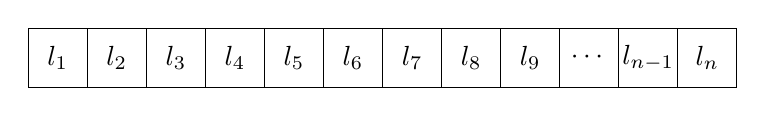
\begin{tikzpicture}[scale=0.75]
        \foreach \x in { 1, 2, 3, 4, 5, 6, 7, 8, 9 } {
            \draw (\x-1,0) rectangle (\x,1);
            \node at (\x-0.5,0.5) {$l_{\x}$};
        }
        \draw (10,0) rectangle (4,1);
        \node at (9.5, 0.5) {$\cdots$};
        \draw (11,0) rectangle (4,1);
        \node at (10.5, 0.5) {$l_{n-1}$};
        \draw (12,0) rectangle (4,1);
        \node at (11.5, 0.5) {$l_{n}$};
        \end{tikzpicture}
        \caption{A sample list $L[1:n]$}
        \label{fig:list-of-boxes}
    \end{figure}
    \vspace*{0pt} \\[0.01pt]
    Let $x$ be the number of elements in $L\left[ \frac{k}{2}:k \right]$ of $\mathbf{\Lambda}$ and to the left of $\sigma_{i}$ in
    $\mathbf{OPT}$'s list. Let $y$ be the number of elements in $L\left[ \frac{k}{2}:k \right]$ of $\mathbf{\Lambda}$ but to the
    right of $\sigma_{i}$ in $\mathbf{OPT}$'s list.
    It is easy to observe that
    \begin{align}
        \mathbf{\Lambda}(\sigma_{i}) &= \frac{k}{2} + x + y + 1 = k + 1 = 2 \cdot (x + y) + 1 \\
        \mathbf{OPT}(\sigma_{i}) &\geq x + 1 - r + \delta
    \end{align}0
    where $\delta$ takes care of any additional exchanges done by $\mathbf{OPT}$. Then we track the change in potential after the
    $i^{th}$ request. If $\mathbf{OPT}$ does not make any other exchanges on the $i^{th}$ request, then the number of inversions in
    $\mathbf{\Lambda}$'s list increases by $x$ and decreases by $y$.
    \begin{align}
        \Delta_{i} &= 2x - 2y + \delta \\
        \implies \mathbf{\Lambda}(\sigma_{i}) + \Delta_{i} &= 2x + 2y + 2x - 2y + 1 + \delta \\
        \label{case-1}
        &= 4x + 1 + \delta \leq \mathbf{4} \cdot \mathbf{OPT}(\sigma_{i})
    \end{align}
    If $\mathbf{OPT}$ moves $L[k]$ to the left, then the number of inversions decreases by at most $x$ and increases by at most
    $\frac{k}{2}$. In this case,
    \begin{align}
        \Delta_{i} &= 2x - 2y + \delta - x + \frac{k}{2} \\
        &= 2x - 2y - x + (x + y) + \delta = 2x - y + \delta \\
        \implies \mathbf{\Lambda}(\sigma_{i}) + \Delta_{i} &= 2x + 2y + 2x - y + 1 + \delta \\
        \label{case-2}
        &= 4x - y + 1 + \delta \leq \mathbf{4} \cdot \mathbf{OPT}(\sigma_{i})
    \end{align}
    where the last inequality follows because $y > 0$, so the inequality holds even after ignoring $y$. \\
    If $\mathbf{OPT}$ moves $L[k]$ to the right, the number of inversions may increase by some $\rho$ but then $\mathbf{OPT}$ also
    pays a cost of $\rho$ for the exchange. So they cancel out in the inequality. \eqref{case-1} and \eqref{case-2} collectively
    prove the inequality in \eqref{cost}. \\
    Adding up the inequality \eqref{cost} for all accesses $i = 1, 2, \hdots, |\sigma|$, we get
    \begin{align}
        \mathbf{\Lambda}(\sigma) = \sum_{i=1}^{|\sigma|} \mathbf{\Lambda}(\sigma_{i}) &\leq \sum_{i=1}^{|\sigma|} 4 \cdot \mathbf{OPT}(\sigma_{i}) - \Delta_{i} \\
        &= 4 \cdot \sum_{i=1}^{|\sigma|} \mathbf{OPT}(\sigma_{i}) - \sum_{i=1}^{|\sigma|} \Delta_{i} \\
        &= 4 \cdot \mathbf{OPT}(\sigma) - \Phi(|\sigma|) + \Phi(0) \\
        \label{final}
        &= 4 \cdot \mathbf{OPT}(\sigma) - \Phi(|\sigma|)
    \end{align}
    where the last quality follows because $\Phi(0) = 0$. \eqref{final} proves the claim since $\Phi(|\sigma|) \geq 0$.
    \hfill $\square$
\end{quote}


\section*{Solution 5.}
We proceed with the proof in a similar fashion as that of online load balancing with restricted assignments where the size of each
job is 1. Let $m$ be the number of machines. Then, we need to prove that the greedy algorithm, $\mathbf{\Lambda}$, is still
$\bigO(\log{m})$-competitive. Let $\mathbf{OPT}(\sigma) = \lambda^{*}$ be the offline optimal solution. A very obvious fact is
that the size of each job
\begin{equation}
    p_{i} \leq \lambda^{*} \text{ for } 1 \leq i \leq |\sigma|
\end{equation}
We denote the load on machine $x$ at some time $t$ by $L_{t}(x)$. By way of contradiction, let us assume that the greedy algorithm
is not $\bigO(\log{m})$-competitive. Let use denote a value slightly larger than 2 by
\begin{equation}
    \mathit{2^{+}} = 2 + \frac{c}{\lambda^{*}} \quad \text{for some } c < \lambda^{*}
\end{equation}
since $\frac{c}{\lambda^{*}} < 1$ by definition (of $c$). Consider the machine $m_{1}$ with the current highest load. Then,
\begin{equation}
    \label{load}
    L_{\text{curr}}(m_{1}) \geq (\mathit{2^{+}} \log{m} + \mathit{2^{+}}) \cdot \lambda^{*}
\end{equation}
Let $J_{1}$ be the set of the minimum number of jobs last assigned to $m_{1}$ such that their total load is more than $2\lambda^{*}$,
i.e. the total load of $J_{1}$ is $2 \lambda^{*} + c$ where $c < \lambda^{*}$. Since $\lambda^{*}$ is the maximum load on any machine
in $\mathbf{OPT}$, there must exist at least one more machine in $\mathbf{OPT}$ (and hence in $\mathbf{\Lambda}$), say $m_{2}$, where
some $k_{1}$ many jobs from $J_{1}$ must be assigned such that their total load is at least $\lambda^{*}$. Let's call this subset $J_{2}$. \\
Consider the time $\tau$ when the first job from $J_{2}$ arrived and was assigned to $m_{1}$ by $\mathbf{\Lambda}$. This must have
happened as $L_{\tau}(m_{1}) \leq L_{\tau}(m_{2})$. But $L_{\tau}(m_{1}) \geq L_{\text{curr}} - (2 \lambda^{*} + c)$, i.e.
$L_{\tau}(m_{2}) \geq L_{\text{curr}} - (2 \lambda^{*} + c)$. Therefore, we conclude that at least two machines with load at least
$L_{\text{curr}} - (2 \lambda^{*} + c)$ exist in $\mathbf{\lambda}$. \\
We now repeat the same argument by considering the jobs responsible for increasing the load on both machines $m_{1}$ and $m_{2}$
from at least $L - 2 \cdot (2\lambda^{*} + c)$ to at least $L - (2 \lambda^{*} + c)$. This is always possible by assuming a sufficiently
large load on machines $m_{1}$ and $m_{2}$. This gives that there are now some $k_{2}$ many jobs, having a total load of at least
$2 \cdot (2 \lambda^{*} + c)$. This means that $\mathbf{OPT}$ needs at least four machines to handle this load, otherwise its answer
would be more than $\lambda^{*}$. \\
Each time we repeat this process, we have shown that the number of machines doubles. We can repeat this argument for some $r$ times until
\begin{align}
    L_{\text{curr}} - r \cdot (2 \lambda^{*} + c) &\leq 2 \lambda^{*} + c \\
    \implies r &\geq \frac{L_{\text{curr}} - 2 \lambda^{*} - c}{2 \lambda^{*} + c}
\end{align}
Now, by \eqref{load}, we have
\begin{align}
    r &> \frac{(\mathit{2^{+}} \log{m} + \mathit{2^{+}}) \cdot \lambda^{*} - (2 \lambda^{*} + c)}{2 \lambda^{*} + c} \\
    &= \frac{\lambda^{*}}{2 \lambda^{*} + c} \left[ \left(2 + \frac{c}{\lambda*} \right) \log{m} + \left( 2 + \frac{c}{\lambda*} \right) \right] - 1 \\
    &= \frac{(2 \lambda^{*} + c) \log{m} + (2 \lambda^{*} + c)}{2 \lambda^{*} + c} - 1 \\
    &= \log{m} + 1 - 1 = \log{m}
\end{align}
The above set of equations mean that there are at least more $2^{r} = m$ machines, which is a contradiction.
Hence, the most heavily loaded machine must also have a load of at most $(\mathit{2}^{+} \log{m} + \mathit{2}^{+}) \cdot \lambda^{*}$.
Since $\frac{c}{\lambda*} < 1$, we can also say that the load will be at most $(3 \log{m} + 3) \cdot \lambda^{*}$. \hfill $\square$


\section*{References}
\begin{enumerate}
    \item Lecture Notes, CSE586 (Monsoon 2023, Dr. Syamantak Das)
    \item \href{http://www.cs.tau.ac.il/~azar/Online-Class2.pdf}{Lecture Notes, Online Algorithms (2011, Yossi Azar)}
\end{enumerate}

\end{document}